下面将介绍逆扩散过程与扩散过程。为了能与『基于扩散的图像生成模型』基本流程形成较好的衔接,所以先介绍逆扩散过程。

\subsection{逆扩散过程}
\label{sec_inverse}

逆扩散过程可以被描述为这样一个过程:从噪声图像中恢复出不带有噪声的图像的过程。为了实现这个目标,在『基于扩散的图像生成模型』中存在多个Denoise过程, 该过程即图\ref{fig_process_of_model}表示的过程。

Denoise过程接收当前的工作步数与上一个Dnoise过程的输出作为输入,输出一张在上一个Denoise输出基础上的部分去噪图,如下图所示。

上图中的每个Denoise过程都由同一个神经网络完成,即一个神经网络即可完成所有的Denoise过程。为了使这样的Denoise网络能完成这样的目标,我们需要大量成对的训练数据。这样的成对数据中应该包含两部分:当前工作步数与工作步数对应的部分去噪图。为了获取上述成对数据以供Denoise网络训练,我们需要扩散过程。

\subsection{扩散过程}

扩散过程可以被描述成这样一个过程:从清晰图像逐步添加噪声直到完全变成噪声图像的过程。为了模拟这种从无噪声到有噪声的过程,在基于扩散的图像生成模型中,通过逐步增加噪声来生成一系列带有不同程度噪声的图像。具体来说,扩散过程从一张清晰图像开始,逐步在多个步骤中加入噪声,最终得到一个完全噪声化的图像,如下图所示\ref{fig_kuosan}。

\begin{figure}[htbp]
    \centering
    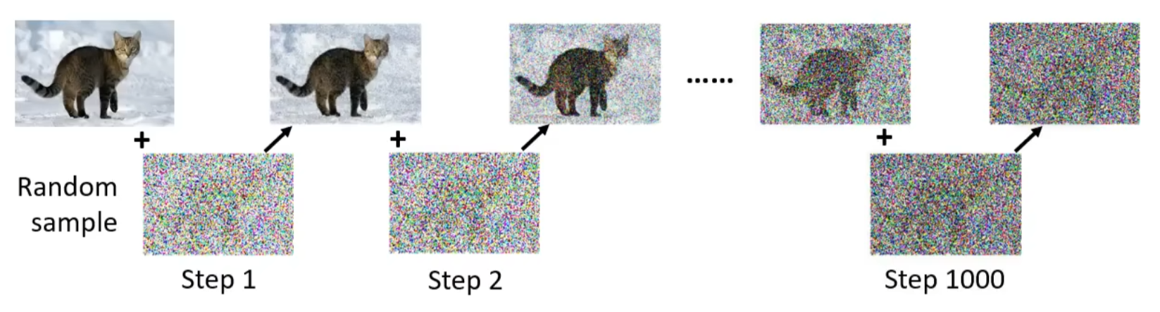
\includegraphics[width=0.8\textwidth]{figs/color/kosan.png}
    \caption{扩散过程}
    \label{fig_kuosan}
\end{figure}

在扩散过程的每一步中,图像中的噪声增加的程度是通过预定义的噪声分布实现的。每个步骤的输出即为下一个步骤的输入,逐步累积噪声直至达到预设的最大噪声水平。

上图中的每个扩散步骤都通过添加高斯噪声来实现,这些高斯噪声是通过一个简单的随机数生成器产生的。为了确保扩散过程能够准确地模拟自然图像中噪声的增加,噪声的分布和强度必须经过精确的设计和调整。

通过这种方式,扩散过程生成了大量的带噪声图像,这些图像用于训练逆扩散过程中的Denoise网络。每对训练数据中的一个部分是一个特定工作步数下的带噪声图像,另一个部分是该步数下去噪后的部分清晰图像。